\documentclass[12pt]{report}
\usepackage[a4paper, top=3cm, bottom=3cm]{geometry}
\usepackage[latin1]{inputenc}
\usepackage{setspace}
\usepackage{fancyhdr}
\usepackage{tocloft}
\usepackage{titlesec}
\usepackage{hyperref}
\usepackage{amssymb}
\usepackage{url}
\usepackage{indentfirst}
\usepackage{graphicx}
\usepackage{listings}
\usepackage{amsmath}
\usepackage[all]{xy}
\usepackage[font=footnotesize, labelfont={footnotesize,footnotesize}, margin=0cm]{caption}
\usepackage{amsfonts}
\usepackage{fixltx2e}
\usepackage{hyperref}
\usepackage{stmaryrd}

\fancypagestyle{plain} {
	\fancyhf{}
	\lhead[\rightmark]{\thepage}
	\rhead[\thepage]{\leftmark}
	\setlength{\parindent}{0pt} 
	\setlength{\parskip}{2ex}
}

\setlength{\parskip}{2ex}

\hypersetup{
    bookmarks=true,   
    unicode=false,
    pdftoolbar=true,  
    pdfmenubar=true,     
    pdffitwindow=false,    
    pdfstartview={FitH},  
    pdftitle={Quotient Containers in Homotopy Type Theory},  
    pdfauthor={Jonathan Sherry},
    pdfnewwindow=true,  
    colorlinks=true,  
    linkcolor=black,  
    citecolor=black, 
    filecolor=black,  
    urlcolor=black  
}

\renewcommand{\filename}[1]{\texttt{#1}}
\newcommand{\function}[1]{\textbf{#1}}
\newcommand{\type}[1]{\texttt{#1}}
\newcommand{\variable}[1]{\textsl{#1}}


\titlespacing{\section}{0pt}{0pt}{0pt}

\begin{document}

\setcounter{page}{-100}
\date{}
\title{\textbf{Quotient Containers in\\ Homotopy Type Theory\\}
Jonathan E. Sherry\\
\vspace{10pt}
    { \large
    \textit{School of Computer Science and Information Technology}\\
    \textbf{University of Nottingham}\\
    }
\vspace{45pt}
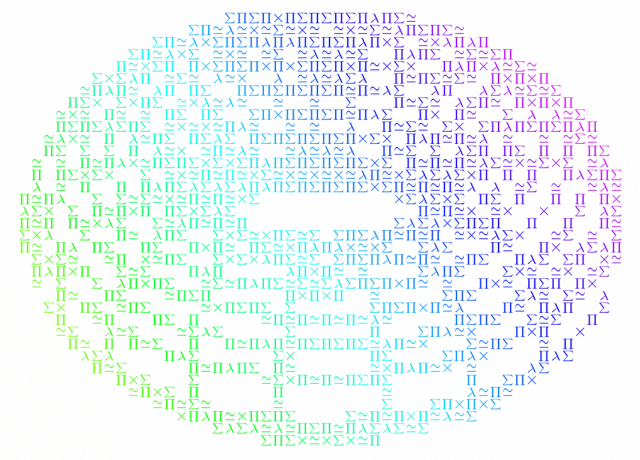
\includegraphics[scale=0.45]{1.png}\\
}
\author{Submitted May 2014 in partial fulfilment of the conditions of\\
the award of the degree of BSc (Hons) Computer Science.\\
\\
I hereby declare that this dissertation is all my own work,\\
except as indicated in the text:\\
\\
Signature \line(1,0){200}\\
Date \line(1,0){40}/\line(1,0){40}/\line(1,0){40}\\
}

\thispagestyle{empty}
\maketitle

\tableofcontents

\pagestyle{fancy}
\pagenumbering{arabic}
\lhead[]{\thepage}
\rhead[\thepage]{}

\part{Introduction}

\chapter{Abstract}


This paper serves to introduce and explain the notions of Martin L\"of Type Theory, Homotopy Type Theory, Containers and Differentiation of Data structures. Using ideas from each of these fields, Quotient Containers are introduced - specifically a multiset container and implmented in \textit{Agda}. The veracity of the implementation is then tested through differentiating a multiset container and concluding that the implementation behaves as one would expect and is true to theory.

\chapter{Acknowledgements}
This study would not have been made possible without the following:
Thorsten\\
Mum, Dad Tony\\
etc.
\chapter{Motivation}

\part{Research}

\chapter{Martin-L\"of Type Theory}
\section{Introduction}
Martin-L\"of type theory is a form of constructive, intuitionistic type theory that is both a programming language and an alternative foundation of mathematics. Devised by Swedish mathematician and philosopher Per Martin-L\"of in 1972, Martin-L\"of type theory (MLTT) serves to provide a set of formal rules and type-theoretic connectives to perform mathematical reasoning.
MLTT is said to be \textit{constructive} and \textit{intuitionistic} as it replaces the classical concept of Truth, with the notion of constructive provability. That is, construction of a mathematical object is proof of its existence. In MLTT, objects are classified by the basal notion of a \textit{type} primitive --- objects can have a certain type and are said to inhabit that type. These structured types can be used to provide a specification for the elements within it, providing a means to reason about objects of that type. For example, from a type:
\begin{center}
$A \rightarrow B$
\end{center}
, the type of functions from type \textit{A} to type \textit{B}, instructions on how to construct an object are implicitly known. In this case, an object of the type $A \rightarrow B$ is formed from an object of type \textit{B}, parametrised by an object of type \textit{A}.

The rigorous rules and predictable nature of objects and types within MLTT afford it strength in formal reasoning. This strength has led to its implementation as a base for a number of languages and proof assistants including Agda \textit{(see chapter 8)}, Epigram and Coq, among others.

This chapter constitutes a brief introduction to key concepts and ideas within Martin-L\"of type theory required for the rest of the text.

\section{Basic Constructions}
\begin{center}
\begin{tabular}{c l}
\textit{A} Type & Declaration of a type \textit{A}.\\
$a : A$ & Object \textit{a} exists and inhabits type \textit{A}. \\
$A \equiv B$ & Type \textit{A} is judgementally equal to type \textit{B}.\\
$ a \equiv b : A$ & \textit{a} and \textit{b} are judgementally equal terms of type \textit{A}.\\
$\Gamma \vdash A$ & A is well-formed in the context $\Gamma$.\\
$\Gamma \vdash a:A$ & \textit{a} is well-formed term of the type \textit{A} in the context $\Gamma$.
\end{tabular}
\end{center}


\section{Type Connectives}
\subsection{Finite Types}
Finite types are those that have a strictly finite, enumerable number of inhabitants. Examples include:
\begin{itemize}
\item the \textbf{0}-type. Otherwise known as the \textit{empty} or \textit{bottom} type, it has no inhabitants and invoking the Curry-Howard isomorphism\footnote{

Discovered by Haskell Curry and William Alvin Howard, the Curry-Howard isomorphism states that there is an equivalence between logic and programming. More formally, there is a syntactic analogy between formal logic and computational calculi.

}, it represents False. An inhabitant of the \textbf{0}-type may be referred to as a \textit{contradiction} as there is no way to prove a contradiction and nor can the \textbf{0}-type be constructed.
\item the \textbf{1}-type. Also called the \textit{unit} type. It has only one inhabitant and invoking the Curry-Howard isomorphism, it represents True. 
\item the \textbf{2}-type. Intended to have exactly two inhabitants: $0_\textbf{2}$ and $1_\textbf{2}$, it could be constructed as \textbf{1} + \textbf{1}. This is the type of Booleans.
\end{itemize}

\subsection{Product Types}
Given types $A,B : \mathcal{U}$, $A \times B : \mathcal{U}$ is the type of their cartesian product where elements of $A \times B$ are pairs $(a,b) : A \times B$ such that $a : A$ and $b : B$. 

\subsection{Coproduct Types}
Given types $A,B : \mathcal{U}$, $A + B : \mathcal{U}$ is the type of their coproduct. Inhabitants of $A + B$ can be constructed with \texttt{inl(a)} : $A + B$ for $a : A$ or \texttt{inr(b)} : $A + B$ for $b : B$.


\subsection{$\Pi$-Types}
$\Pi$-types, also known as dependent product type, is a type whose inhabitants are functions whose codomain is dependent on the domain to which the function is applied. It can be regarded as the cartesian product over a type.\\
Given a type \textit{A} : $\mathcal{U}$ and a family \textit{B} : \textit{A} $\rightarrow$ $\mathcal{U}$, we can construct the type of dependent functions:
\begin{center}
$ \prod_{(x:A)}^{} B(x) : \mathcal{U} $
\end{center}
For a constant family \textit{B}, this is judgementally equal to a function \textit{A} $\rightarrow$ \textit{B}.\\
Polymorphic functions are an example of a dependent type element. A polymorphic function would be of the type:
\begin{center}
$ \prod_{(A:\mathcal{U})}^{} A \rightarrow B $
\end{center}
Invoking the Curry-Howard isomorphism, $\Pi$-types represent implication and universal quantification.


\subsection{$\Sigma$-Types}
$\Sigma$-types, or dependent pair types, are types where the latter component of a pair depends on the former. It is analogous to an indexed sum over a given type. 
Given a type \textit{A} : $\mathcal{U}$ and a family \textit{B} : \textit{A} $\rightarrow$ $\mathcal{U}$, we can construct the type of dependent pair functions:
\begin{center}
$ \sum_{(x:A)}^{} B(x) : \mathcal{U} $
\end{center}
For a constant family \textit{B}, this is judgementally equal to the cartesian product type: ($A \times B$).
Invoking the Curry-Howard isomorphism, $\Sigma$-types represent conjunction and existential quantification.
\subsection{Identity Types}
Identity or equality types are of the form $a =_A b$ such that $a : A$ and $b : A$. Given a type $A : \mathcal{U}$ and elements $a,b : A$ we can form type $a =_A b : \mathcal{U}$ in the same universe. There is only one inhabitant of this type --- the proof of reflexivity:
\begin{center}
 \texttt{refl} : $\prod_{(a:A)}^{} (a =_A a) $
\end{center}
\texttt{refl} states that all elements in \textit{A} are equal to themselves. This means that if \textit{a} and \textit{b} are judgementally equal, we also have a witness of \texttt{refl},  \texttt{refl\textsubscript{a}} : $(a =_A b)$.
\subsection{Inductive Types}
Inductive types are those that includes a constructor that encodes how to create new elements of the type. Normally, there will be a base case and an inductive case. A good example of this is an inductive definition of the natural numbers. Elements of type $\mathbb{N} : \mathcal{U} $ are constructed with $0 : \mathbb{N} $ and $successor : \mathbb{N} \rightarrow \mathbb{N}$.
\subsection{Universes}
A universe, $\mathcal{U}$, is a type whose elements are types. To avoid Russell's paradox\footnote{
In 1901, Bertrand Russell used this paradox to derive a contradiction in Cantor's naive set theory. The paradox is as follows: "Let R be the set of all sets which are not members of themselves. Then R is neither a member of itself nor not a member of itself."\cite{rp} Type theory was introduced by Russell as a solution to this problem.
}, universes are ordered in a heirarchy. That is, $\mathcal{U}_0 : \mathcal{U}_1$, $ \mathcal{U}_1 : \mathcal{U}_2$... Universes are \textit{cumulative}, meaning all elements of the $i^{th}$ universe are also elements of the $(i+1)^{th}$ universe. When we declare a type, we say implicitly that it inhabits some universe $\mathcal{U}_i$.

\subsection{Propositions as Types}
Using the types above, it is possible to construct types that represent logical propositions, that is, logical sentences with a truth value, as such:
\begin{center}
\begin{tabular}{|c|c|}
\hline 
\textbf{Logic} & \textbf{Type Theory} \\ 
\hline
True & \textbf{1} \\ 

False & \textbf{0} \\ 

\textit{A} and \textit{B} & \textit{A} $\times$ \textit{B} \\ 

\textit{A} or \textit{B} & \textit{A} + \textit{B} \\ 

If \textit{A} then \textit{B} & \textit{A} $ \rightarrow $ \textit{B} \\  

\textit{A} iff \textit{B} & (\textit{A} $ \rightarrow $ \textit{B}) $\times$ (\textit{B} $\rightarrow$ \textit{A})  \\ 

Not \textit{A} & \textit{A} $ \rightarrow $ \textbf{0} \\ 

For all $ x : A, P(x)$ is true & $\prod_{x : A}P(x)$\\

There exists $ x : A$ such that $P(x)$ is true & $\sum_{x : A}P(x)$\\

\hline 
\end{tabular} 
\end{center} 
\section{Equality proofs form a groupoid?}


\chapter{Homotopy Type Theory}
\section{Introduction}
Homotopy type theory is a new branch of mathematics that came about after a special year on \textit{Univalent Foundations of Mathematics} during 2012 and 2013 at The Institute for Advanced Study, Princeton. Organised by Vladamir Voevodsky, Thierry Coqand and Steve Awodey, the \textit{Univalent Foundations} program sought to explore implications of Voevodsky's \textit{Univalence Axiom}, $(A = B) \simeq (A \simeq B)$, that is ``identity is equivalent to equivalence. In particular, one may say that `equivalent types are identical'."\cite{hott}.

Homotopy type theory, an amalgam of type theory; homotopy theory and higher dimensional category theory, is \textit{intentional, dependent} type theory with the \textit{Univalence Axiom} forming the basis of its \textit{structural identity principle}. Formally, this means that
\begin{center}
$ (A \cong_C B) \rightarrow Id_C(A,B) $
\end{center}
where \textit{C} is the type of structured objects with arbitrary signature, $ (A \cong_C B)$ is the type of isomorphisms between \textit{A} and \textit{B} and $Id_C(A,B) $ is the type of objects that witness the identification of \textit{A} with \textit{B}. In other words, \textbf{\textit{Isomorphic structures can be identified}}.

The interpretation of types as structured objects also means that it is possible to apply type-theoretic logic to other structured objects --- namely topological objects, leading to a homotopical interpretation and the ability to reason about homotopy theory using type theory. This homotopical interpretation of types coupled with the \textit{Univalence Axiom} is the basis of homotopy type theory.

\pagebreak

\section{Key Concepts in Homotopy Type Theory}
The fundamental idea behind homotopy type theory is the marriage between Martin-L\"of type theory and homotopical notions. The following uses the languages of type theory, category theory and homotopy theory to present concepts in Homotopy type theory. 
\subsection{Types and their Inhabitants}
\subsubsection{Types as spaces}
In a homotopical interpretation, types are regarded as topological spaces and terms of a type are represented by points in a space.
\subsubsection{Types as $\infty$-Groupoids}
In algebraic topology, a (pointed\footnote{

A pointed topological space is a space $X$ such that it has a distinct basepoint $x_0 \in X$. This basepoint will often dictate the \textit{fundamental group}.

}) space has an associated group that stores information about the `basic shape' of the space. More formally, it stores information on when two paths, beginning and ending at a basepoint can be continuously deformed onto one another. Naturally, it follows that for homeomorphic spaces, this group will be the same. This group is known as the \textit{fundamental group}.

In homotopy theory, every space has a \textit{fundamental $\infty$-groupoid} whose \textit{k}-morphisms (morphisms between morphisms at level \textit{k}) are the \textit{k}-dimensional paths in the space. Homotopy type theory views types as having the structure of this \textit{fundamental $\infty$-groupoid}. This can be seen through iterating the identity type in the following way: given an identity type $a =_A b$ we can consider the type of identified elements : $c =_{(a =_A b)} d$, that is, identifications between identifications and so on.

This structure is analogous to continuous paths of a space and the homotopies between them, in other words, an $\infty$-groupoid. This groupoid model of Martin-L\"of type theory has far reaching implications in higher category theory as groupoids can be modelled as small categories in which all morphisms are isomorphic.

\subsection{Equality}
Given the above, it is consistent to interpret identity types as paths. Thus, for an element $p : a =_A b$, a path $ p : a \leadsto b $ is said to exist between a and b in the space of A. For two elements of the same identity type i.e. for $p,q : a =_A b$, paths are said to be parallel as they have the same start and end points. Thus, it follows that an element of the type $c =_{(a =_A b)} d$ represents a homotopy --- or a morphism between morphisms. This can also be thought of as a 2-dimensional path in \textit{A}. Similarly, the next iteration, the type of identifications between identifications between identifications can be thought of as a 3-dimensional path or a morphism between morphisms between morphisms.
\begin{center}
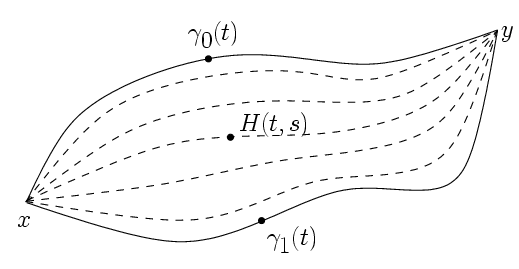
\includegraphics[scale=0.5]{./2.png}\\
\small{\textit{Homotopy between two curves: the curves\\ $\gamma_0$ and $ \gamma_1$ are homotopic by the homotopy $H$}}
\end{center}
In the image above, $\gamma_0, \gamma_1$ could be considered of the type $x = y$ for some space.

\subsection{Functions}
Functions are represented by continuous mappings between spaces. For example, a function $f : A \rightarrow B$ represents a continuous mapping from space \textit{A} to space \textit{B}. Functions can be identified if they are homotopic.

Functions also behave functorially on paths, that is, all functions are continuous and preserve paths.


\subsection{Dependent types}
Dependent types are represented by a fibration - a mapping from a base space to a total space.

\subsection{Higher Inductive Types}
\subsubsection{Multisets as a HIT}
\begin{center}

\end{center}




\section{Summary}

The following table summarises the different interpretations of analogous concepts in the languages of type theory, logic, Zermelo-Fraenkel set theory and homotopy type theory:

\begin{center}
\begin{tabular}{| c | c | c | c |}
\hline
\textbf{Type Theory} & \textbf{Logic} & \textbf{ZFC} & \textbf{Homotopy Theory}\\
\hline
\textbf{0} & $\bot$ & $\varnothing$ &$\varnothing$\\
\textbf{1} & $\top$ & \{$\varnothing$\} &*\\
\textit{A} & proposition & set & topological space\\
$a : A$ & proof & element & point\\
$B(x)$ & predicate & family of sets & fibration\\
$b(x) : B(x)$ & conditional proof & family of elements & section\\
$ Id_A $ & equality & \{$ (x,x) | x \in A $\} & path space $A^{\textit{I}}$\\
$A + B$ & $A \vee B$ & disjoint union & coproduct\\
$ A \times B$ & $A \wedge B$ & set of pairs & product space\\
$A \rightarrow B$ & $A \Rightarrow B$ & set of functions & function space\\
$ \sum_{(x:A)}^{} B(x) $ & $\exists x:A, B(x) $ & disjoint sum & total space\\
$ \prod_{(x:A)}^{} B(x) $ & $\forall x:A, B(x) $ & product & space of sections\\
\hline
\end{tabular}
\end{center}


\chapter{Containers}
\section{Introduction}
\section{Definition}
A unary container is defined as a pair $ (S \rhd P) $ where:
\begin{enumerate}
\item $S : Set$ and elements of $S$ are the \textit{shapes} of the container.
\item $P : Set \to Set$ and for $s : S$, elements of $P(s)$ are the \textit{positions} of \textit{s}.
\end{enumerate}

\subsection{List Container}
As an example, we define a list container, $Con_{List}$ for conventional lists over a type \textit{A}:
\begin{center}
$ L(A) \simeq 1 + A \times L(A) $
\end{center}
or in Agda:
\begin{verbatim}
                 data List (A : Set) : Set where
                      Nil : List A
                      Cons : A -> List A -> List A
\end{verbatim}
 $Con_{List} = (S \rhd P) $ such that \textit{S}, the set of shapes, is $\mathbb{N}$, the set of natural numbers and \textit{P}, the family of positions is $Fin(-)$. The functor $\llbracket Con_{List} \rrbracket$ maps a set to the set of finite sequences in A.


\section{Category of Containers}
The category of containers is composed of containers as objects and container morphisms.
A container can be interpreted as an endofunctor (a categorical mapping from a category to itself):
\begin{center}
$\llbracket S \rhd P\rrbracket : Set \to Set$\\
$ \llbracket S \rhd P\rrbracket X = \Sigma s : S. P s \to X $
\end{center}
and given containers $ (S \rhd P)$ and $ (T \rhd Q)$ morphism $ f \rhd r $ is given by:
\linebreak
\linebreak
$Mor_{Con}(S \rhd P),(T \rhd Q) = $
\begin{center}
$ \sum_{f : S \to T} r : \prod_{x \in S} Q(f(x)) \to P(x)$
\end{center}
Pictorally, this is represented as:
\begin{center}
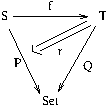
\includegraphics[scale=1]{cm.png}
\end{center}
These container morphisms give rise to natural transformations, morphisms of functors. Given containers $ (S \rhd P)$ and $ (T \rhd Q)$, and a container morphism $ (f , r) : (S \rhd P) \to (S \rhd P)$ we can define a natural transformation:
\begin{center}
$ \llbracket f,r\rrbracket : \llbracket S \rhd P\rrbracket \Rightarrow \llbracket T \rhd Q\rrbracket$ \\
$  \llbracket f,r\rrbracket (s,p) = (f(s),p \circ r_s) $
\end{center}


\section{Quotient Containers}
\subsection{Definition}
Quotient containers are containers furnished with an equivalence relation. More formally, a quotient container $S \rhd P/G$ is defined as a container $S \rhd P$ and for each shape $s$ in $S$, a set of isomorphisms $G(s)$. This set of isomorphisms can be seen as some subgroup of the automorphism group of $P(s)$.

 From this definition, it follows that all containers are degenerate quotient containers where $G(s)$, the set of isomorphisms, is the empty set. 

\subsection{Extention}
The extention of a quotient container $S \rhd P/G$ is a functor:
\begin{center}
$T_{S \rhd P/G} : Set \rightarrow Set$\\
$T_{S \rhd P/G}(x) = \Sigma s:S.(P(s) \rightarrow X)/\sim_{s}$, such that\\
\end{center}
$\sim_{s}$ is the equivalence relation on the set of functions $P(s) \rightarrow X$, such that
\begin{center}
$f \sim f'$ iff $\exists g \in G(s)$ where $f' = f \circ g$
\end{center}

\chapter{$\delta$ for Data}
The idea of differentiation of parametric datatypes was introduced by Conor McBride in 2001. Expanding on Gerard Huet's \textit{Zipper} data structure\cite{zipper}, McBride established that the differential of a type is the \textbf{\textit{type of its one hole contexts}}. That is, if we take an arbitrary type parameterised over a type $X$, removing an item of this type $X$ from the data structure and replacing it with a `hole' or empty element will yeild its \textit{one hole context}. Replacing this hole with an element of type $X$ will produce the original type. This can be easily represented pictorally:
\begin{center}
DIAGRAM
\end{center} 
This chapter borrows its title from a 2005 paper by Abbott, Altenkirch, Ghani and McBride that serves to explain and analyse derivatives of data structures.
\section{Differentiating Data Structures}
The formalisation of the differentiation of data types is given by way of example. To find the differential of a type $FX = F_{1}X \times F_{2}X$, we must find the type of its one hole context. In the case of this type, a hole is:
\begin{itemize}
\item a hole in $F_{1}$, or
\item a hole in $F_{2}$.
\end{itemize}
Thus, the type of $\delta F$, is the differential of $F_{1}$ and $F_{2}$ or the differential of $F_{2}$ and $F_{1}$. More formally,
\begin{center}
$\delta F \simeq \delta F_{1} \times F_{2} + F_{1} \times \delta F_{2} $
\end{center}
We may picture this as:
\begin{center}
DIAGRAM
\end{center}
It is worth comparing the rule for differentiating this type $F$ with the product rule from classical, differential calculus:
\begin{center}
$\delta F \simeq \delta F_{1} \times F_{2} + F_{1} \times \delta F_{2} $\\
c.f.\\
$\frac{d}{dx} (u \cdot v)= \frac{dv}{dx} \cdot u + v \cdot \frac{du}{dx}$
\end{center} 
On observation, it would appear that these are analogous. Indeed they are and all usual rules and laws of differential calculus such as the chain rule, product rule, et cetera apply to all parametric type contructors. This is fully investigated in (Abbot, 2003).
\subsection{Differentiation of a List}
By way of additional example for further illumination, we differentiate a list. Given the list functor,
\begin{center}
$L(X) \simeq 1 + X \times L(X)$,
\end{center} 
we may think of its type of one hole contexts to be the type where a hole is placed at an arbitrary position in a non-empty list. A list with a hole placed in the centre would give us two equally sized lists, while edge cases, in the form of holes at the head and tail of the list, would yeild a non-empty list and an empty list. Thus, our intuition tells us that the differential of a list is two lists. More formally, this is expressed as:
\begin{center}
$\delta L(X) \simeq L(X) + X \times \delta L(X)$
\end{center}
\section{Differentiating Containers}
Similar to the notion of ``types of one hole contexts", the derivative of a container is the container that comprises all posible ways to remove a position from that container.\\
For a container $(S \rhd P)$,
\begin{center}
$\delta (S \rhd P) = (s,p) \Sigma s : S . P(s) \rhd \Sigma p':P(s),p \neq p'$.
\end{center}
Considering the extention of a container, $T_{S \rhd P/G}(x) = \Sigma s:S.(P(s) \rightarrow X)/\sim_{s}$, we may express the differentiation of a container as:
\begin{center}

\end{center}


\subsection{Differentiation of a List Container}
\begin{center}
$L = (S \rhd P)$ such that $S = \mathbb{N}, P = Fin(-)$\\
$\delta(L) = \Sigma n : \mathbb{N}, p: Fin(n) \rhd \Sigma p' : Fin(n), p \neq p'$\\
$\simeq $\\
$(m,n): \mathbb{N} \times \mathbb{N} \rhd Fin(n) + Fin(n)$\\
$= (L \times L)$\\
\end{center} 


\chapter{Agda}
Agda is a programming language come proof assistant based on Martin-L\"of Type Theory (See \textbf{Chapter 4}).







\part{Quotient Containers in Homotopy Type Theory}
\chapter{Implementation}
\begin{center}
$S_M : Type_1$\\
$e : \mathbb{N} \to S_M$\\
$\epsilon : Fin(m) = Fin(n) \to e(m) = e(n) $\\
\end{center}
And family:
\begin{center}
$P_M : S_M \to Set$\\
$P_M(e(n)) = Fin(n)$\\
$P_M(\epsilon(\alpha)) = transport(Fin, \alpha)$\\

\part{Conclusions}

\chapter{Evaluation}

\chapter{Conclusion}

\chapter{Further Work}

\cleardoublepage
\phantomsection
\addcontentsline{toc}{chapter}{Bibliography}

\begin{thebibliography}{10}

\bibitem{MLTT}
  Per Martin-L\"of,
  \emph{Intuitionistic Type Theory},
  1980

\bibitem{pMLTT}
  Bengt Nordstr\"om, Kent Petersson, Jan M. Smith,
  \emph{Programming in Martin-L\"of's Type Theory, An Introduction},
  1990

\bibitem{hott}
  The Univalent Foundations Program, Institute for Advanced Study,
  \emph{Homotopy type theory: Univalent foundations of mathematics}.
  2013.

\bibitem{hott1}
  Michael Abbott, Thorsten Altenkirch, Neil Ghani,
  \emph{Constructing Strictly Positive Types}.
  2004.
  
\bibitem{hot2}
  Michael Abbott, Thorsten Altenkirch, Neil Ghani, Connor McBride,
  \emph{$\delta$ for Data, Differentiating Data Structures}.
  2005.

\bibitem{hott3}
  Hakon Robbestad Gylterud,
  \emph{Symmetric Containers (MSc Thesis)}.
  2005.
  
\bibitem{;luhg;}
  Thorsten Altenkirch, Paul Levy, Sam Staton,
  \emph{Higher Order Containers}
  2010.
  
\bibitem{hott4}
  http://homotopytypetheory.org/
  
\bibitem{rp}  
  http://mathworld.wolfram.com/RussellsAntinomy.html
  
\bibitem{zipper}
  http://en.wikibooks.org/wiki/Haskell/Zippers

\end{thebibliography}
\cleardoublepage
\phantomsection
\addcontentsline{toc}{chapter}{Appendix}

\chapter{Appendix}

\end{document}